\addchapheadtotoc
\chapter{Results and Discussion}
In this chapter we introduce the experiments conducted in this work  with a discussion of the results. Most of these experiments were on a synthetic graph dataset created based on what's called the stochastic block model (SBM). This generative model is considered since we can control the difficulty of the graph classification problem it introduces and since it is widely used to model real world datasets \citep{SBM}. \newline
One by one, we analyze how our algorithm $GSA-\varphi_{OPU}$, followed by a linear support vector machine model (SVM), is affected by the following parameters: the sampling technique, the number of samples $s$, the graphlet size $k$ and the number of random features $m$.
Then we benchmark this algorithm against state-of-the-art methods: graphlet kernel and graph convolutional networks (GCN). In addition, we benchmark it to $GSA-\varphi_{Gs}$.
In the end, we show some experiments that were done on one real world dataset named \emph{DD} dataset. However, we start now by a general introduction to the generative SBM model. 
\section{Stochastic block model (SBM) dataset}
SBM is commonly known in social sciences to model group structures in friendship graph networks\citep{SBM}. The basic idea here is that nodes  are clustered into many groups, called communities, within the same graph. Then, the neighborhood relations of a node, edges to neighbor nodes, are generated such that nodes in the same community have similar neighbor patterns either to nodes in the same community or to nodes in other communities. \newline
Formally, to generate a graph $\G=(\V,\E)$ of size $v$, the following parameters should be given: The number of communities $\eta$ in the graph, node labels $\{b_1 , \ldots ,b_v\}$ such that node $u$ belongs to community $b_u$, and edge probability matrix $\mathbf{P}=(p_{i,j})_{i,j\in\{1,\ldots, \eta\}}$.
Then the graph is generated by independently adding an edge between any two pair of nodes $(u_1,u_2)$ with probability $p_{b_{u_1} , b_{u_2}}$. \newline
\begin{figure}[H]
\centering
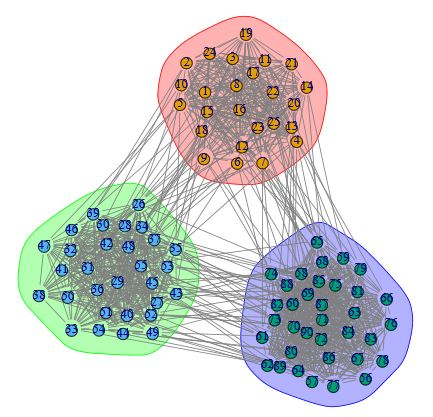
\includegraphics[scale=0.5]{Dissertation/figs/SBM.JPG}
\caption[Visualization of an SBM-based graph example]{An example of a graph generated using SBM model, the graph has 90 nodes divided into three communities of size 25, 30 and 35 nodes. An edge between two nodes within the same community has a probability 0.8, while it has a probability 0.5 if the two nodes belong to different communities.}
%Source:
\label{fig:SBM_example}
\end{figure}
An easy thing to compute here is the average number of edges $\mu$ incident to a node $u$:
\begin{equation}
    \mu_u=\Big[\sum_{b_i\neq b_u} p_{b_u,b_i}*(\#u'\in \V, b_{u'}=b_i \} )\Big]+p_{b_u,b_u}*(\#\{u'\in \V_\G, b_{u'}=b_u \}-1 )
\end{equation}
\subsection{Dataset setup}
In our case and almost in every experiment, unless otherwise mentioned, the SBM dataset consists of 300 graphs, 240 as a training set and 60 as a test set. Each graph has $v=60$ nodes divided equally between six communities $\eta=6$. Moreover, since we are interested in graph 2-classes classification, graphs are divided into two classes based on two different values of the matrix $\mathbf{P}$. But the two matrices have something in common:  $p_{1,1}= p_{2,2} = p_{in}$ and it is obvious that  $p_{1,2}=p_{2,1}=p_{out}$ too, as we want an indirect graphs dataset as indicated previously.\newline
Thus, the first class of graphs corresponds to a fixed pair ($p_{in,1}, p_{out,1}$) and similarly the second   corresponds to ($p_{in,2}, p_{out,2}$). \newline 
In order to prevent the two classes from being easily discriminated by the average degree of nodes in the graph as a feature, the two pairs of probabilities are always chosen so that any node in any graph in any class has the same expected average degree equal to 10. For simplicity, we refer to $r=(p_{in,1}/p_{in,2})$ with inter-classes similarity parameter. Where the closer to one $r$ is, the more similar both classes are, based on the average degree condition,  and thus the harder it is to discriminate them. One notes here that the only parameter that is left to be modified in the experiments is $r$ .


\section{$GSA-\varphi_{OPU}$ behavior with respect to number of samples $s$}
We did two experiments here: the first one is to compare the graphlet distributions introduced by both uniform and random walk sampling, while the second one is to determine the minimum number of samples needed to classify both classes with high test accuracy, or what should be called here validation accuracy.\newline
\subsection{Uniform sampling Vs. random walk sampling}
We generated a graph $\G$ by SBM with a randomly chosen pair $(p_{in},p_{out})$, then we did the following: exhaustive enumeration of all size-5 graphlets in $\G$,  sampling 2000 graphlets of the same size with uniform sampling, then sampling other 2000 graphlets using random walks. For each case, we matched samples to their corresponding graphlet, considering \emph{graphlets without repetition}, to have three graphlet histograms at the end as shown in Fig. \ref{fig:graphlet_hist}. 


\begin{figure}[H]
\centering
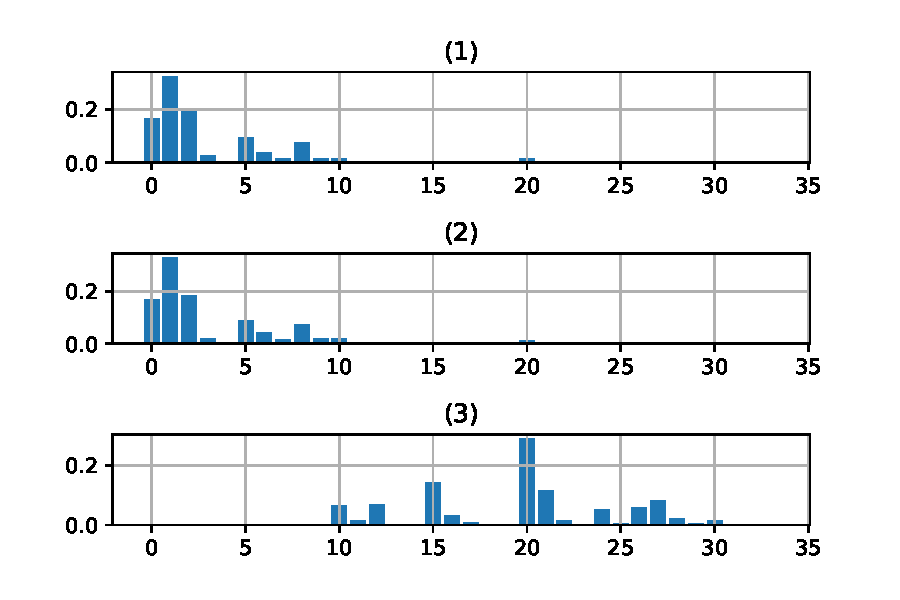
\includegraphics[scale=0.5]{Dissertation/figs/class0_hist.pdf}
\caption[Graphlet histograms of uniform and random walk sampling techniques]{Size-5 graphlet histograms of an SBM random graph, with respecting the isomorphism test. (1): With exhaustive enumeration of all graphlets. (2): 2000 samples with uniform samples. (3): 2000 samples using random walks. }
%Source:
\label{fig:graphlet_hist}
\end{figure}
We see from the results that unlike random walks, uniform sampling is the method to be considered as a sampling technique to approximate graphlet kernel, since it introduces the same histogram as the one used in graphlet kernel. 
\subsection{Varying the number of samples $s$}
experiment setup: number of random features $m=5000$, inter-class similarity $r=2$, input: adjacency matrix $\mathbf{A}$, and sampler: uniform sampling. These parameters were chosen after many experiments to make sure that the 2-classes can be efficiently classified with sufficiently large $s$ and large $k$. Then for graphlet sizes $k\in\{4,5,6\}$, we tried different number of samples and plotted the test accuracy as shown in Fig. \ref{fig:varying_samples_num}.\newline
Results show that even with large number of samples, the algorithm will not perform well if the graphlet size is small as in $k=4$ case. To understand this we can consider the critical case when we use $k=1$ between two graphs, which means that we count how many nodes there are in each. Obviously this is a redundant choice since such graphlets don't provide a lot of information on how nodes are structured and connected in the graph. Thus, for each application, we must choose large $k$ so that graphlets include discriminative patterns not useless ones.
\begin{figure}[H]
\centering
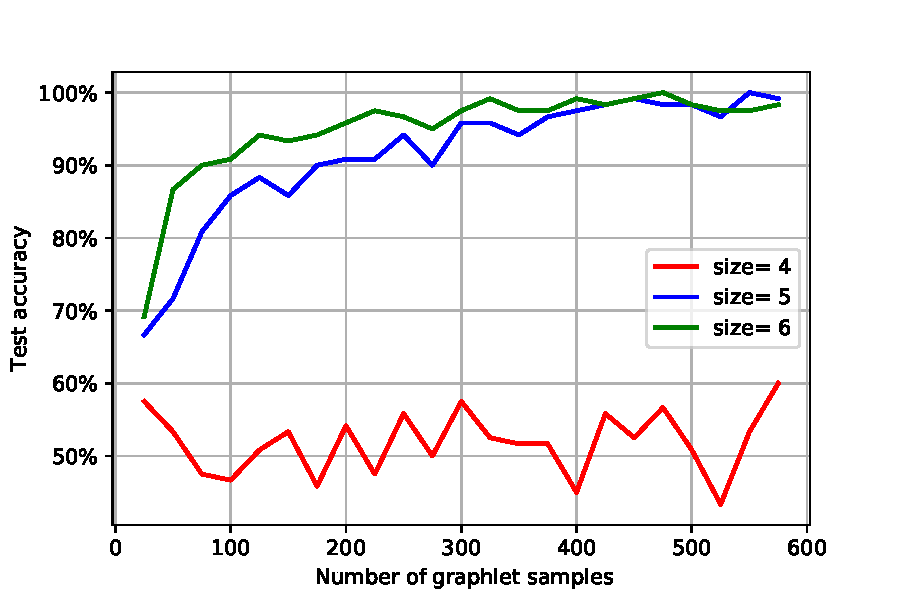
\includegraphics[scale=0.5]{Dissertation/figs/samples_num.pdf}
\caption[$GSA-\varphi_{OPU}$ behavior with respect to number of samples $s$]{$GSA-\varphi_{OPU}$ behavior with respect to number of samples $s$. With $r=2,$, $m=5000$, $k\in\{4,5,6\}$, input: $\mathbf{A}$ and sampler: uniform sampling technique.}
%Source:
\label{fig:varying_samples_num}
\end{figure}
The second note is that in this experiment and even in the next ones, we don't have access to apply the kernel which corresponds to OPUS' random features. That's why we cannot get sure that these results meets the concentration inequalities in chapter\ref{chapter:fast_algorithm}. However, we see that for $k\in\{5,6\}$, test accuracy increases as  $s$ increases, \emph{i.e.} this implies that with higher number of samples $GSA-\varphi_{OPU}$ performance converges to the corresponding mean kernel with higher probability.




\section{$GSA-\varphi_{OPU}$ behavior with respect to the number of random features $m$}
In this experiment we explore the role of random features number $m$ in our algorithm. 
Experiment setup: inter-class similarity: $r=1.1$, graphlet size: $k=6$, sampler: samples number $s=2000$, input: adjacency matrix $\mathbf{A}$, and uniform sampling.
\begin{figure}[H]
\centering
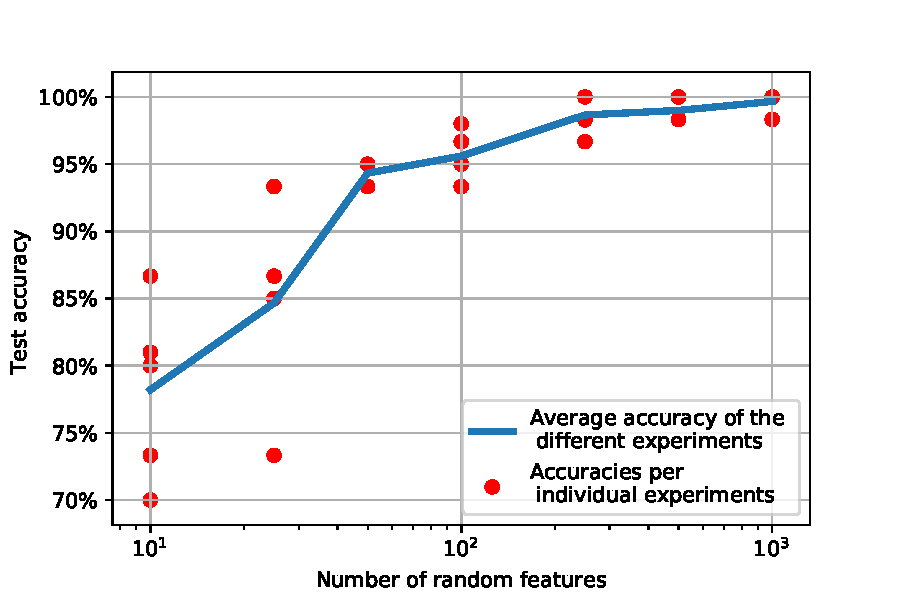
\includegraphics[scale=0.5]{Dissertation/figs/LightON_adj_SBM_varying_RF.PDF}
\caption[$GSA-\varphi_{OPU}$ behavior with respect to number of random features $m$]{$GSA-\varphi_{OPU}$ behavior with respect to number of random features $s$. With  $r=1.1$, $k=6$, $m=5000$, input:$\mathbf{A}$ and sampler: uniform sampling technique. For every value of $m$, the experiment is done five times (red dots), then the $5$ resulted accuracies are averaged (blue curve).}
\label{fig:varying_random_features}
\end{figure}
In addition, for every value of $m$, we applied our algorithm $5$ times on the dataset we have, and then the average of test accuracies is computed. Results are shown in Fig. \ref{fig:varying_random_features}, where we can  see that when $m$ grows, the average test accuracy gets higher, \emph{i.e.} we approximate the performance of the original mean kernel. Even further, as $m$ increases, the 5 experiments provide lower-variance accuracies, which is compatible with the concentration inequalities in chapter \ref{chapter:fast_algorithm}.

\section{testing $GSA-\varphi_{OPU}$ discrimination power}
\begin{figure}[H]
\centering
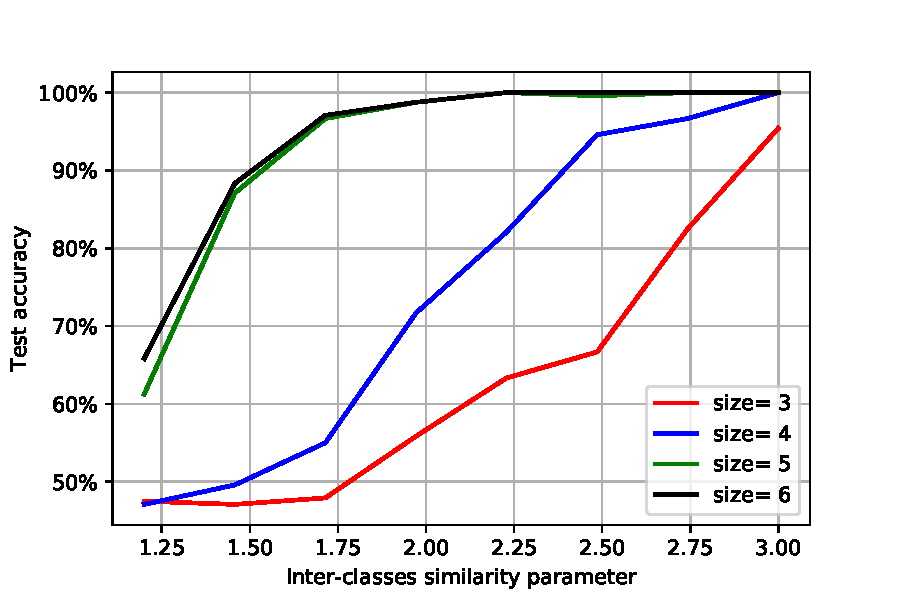
\includegraphics[scale=0.7]{Dissertation/figs/LightOn_adj_SBM_Similarity_graphlet_size.pdf}

\caption[Classification test accuracy as a function of Inter-classes similarity parameter ]{Classification test accuracy with respect to Inter-classes similarity parameter when the number of random features is fixed to 5000 but with different sizes of the graphlet to be sampled. The SVM model is trained on SBM 240-sized labeled dataset. Per graph G, 2000 graphlet samples (Uniform sampling) of the corresponding size are considered to compute its features map $\phi(G)$.}
%Source:
\label{fig:LightOn_adj_SBM_mult_factor}
\end{figure}

\begin{figure}[H]
\centering
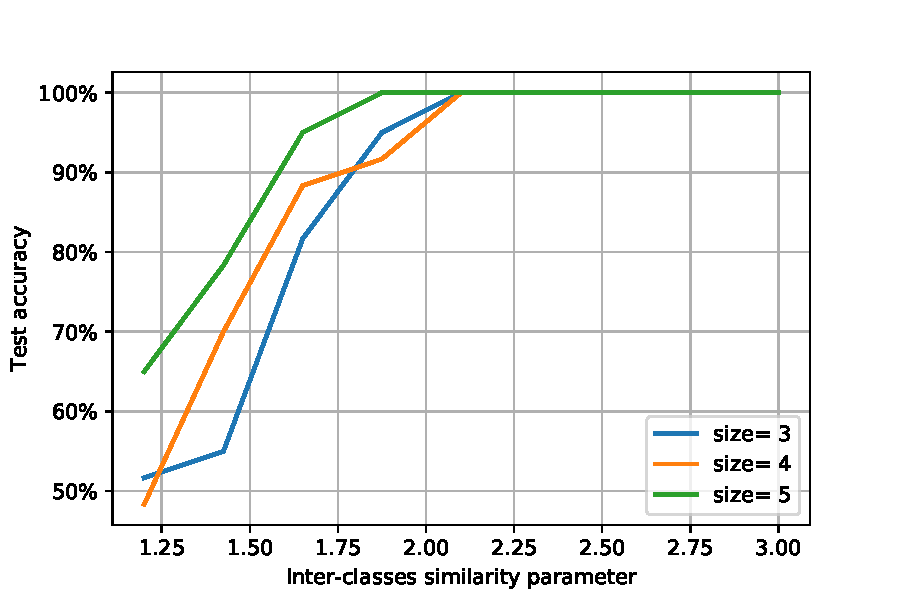
\includegraphics[scale=0.7]{Dissertation/figs/LightOn_adj_SBM_similarity_graphlet_size_RW.pdf}
\caption[Classification test accuracy as a function of Inter-classes similarity parameter ]{Classification test accuracy with respect to Inter-classes similarity parameter when the number of random features is fixed to 5000 but with different sizes of the graphlet to be sampled. The SVM model is trained on SBM 240-sized labeled dataset. Per graph G, 2000 graphlet samples (Random Walk sampling) of the corresponding size are considered to compute its features map $\phi(G)$. This experiment is done to check if the uniform sampling technique is the reason behind the gap between accuracy curves of graphlet sizes 4 and 5 in Fig. \ref{fig:LightOn_adj_SBM_mult_factor} }
%Source:
\label{fig:LightOn_adj_SBM_multfactor_RW}
\end{figure}

\section{Benchmark $GSA-\varphi_{OPU}$ against $GSA-\varphi_{Gs}$}

\section{Benchmark $GSA-\varphi_{OPU}$ against graphlet kernel}
\begin{figure}[H]
\centering
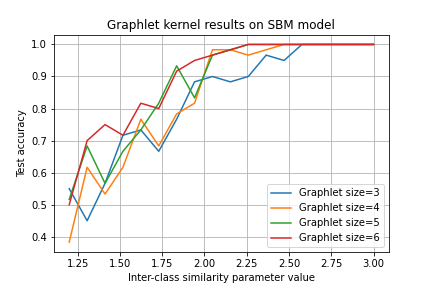
\includegraphics[scale=0.7]{Dissertation/figs/graphlet_kernel_SBM_accuracy.png}
\caption[Graphlet kernel classification test accuracy as a function of Inter-classes similarity parameter]{Graphlet kernel classification test accuracy with respect to Inter-classes similarity parameter $r$. where per graph G, 2000 graphlet samples are considered to compute its graphlet spectrum vector. }
%Source:
\label{fig:graphlet_kernel_SBM}
\end{figure}

\section{Benchmark $GSA-\varphi_{OPU}$ against graph convolution networks}
\begin{figure}[H]
\centering
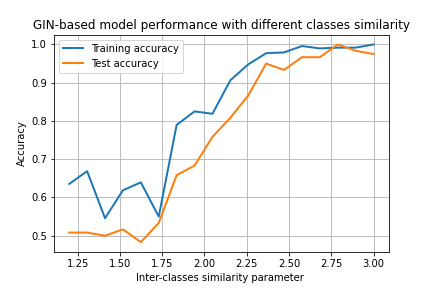
\includegraphics[scale=0.7]{Dissertation/figs/GNN_GIN.png}
\caption[GCN model's classification test accuracy as a function of Inter-classes similarity parameter ]{GCN model's classification test accuracy with respect to Inter-classes similarity parameter. The  model is trained on SBM 240-sized labeled dataset.}
%Source:
\label{fig:GCN_GIN_SBM_multfactor_RW}
\end{figure}

\section{$GSA-\varphi_{OPU}$ results on DD dataset}
\section{Conclusion and future work}





